%----------------------------------------------------------------------------
\chapter{Elméleti összefoglaló}
%----------------------------------------------------------------------------

\section{Hagyományostól az end-to-end-ig}

A hagyományos ASR-ok (automatikus beszédfelismerők) több elemből álló, összetett rendszerek, melyek manapság igen pontosan meg tudják állapítani mi volt az eredetileg elhangzott szöveg, és leképezik azt írásos formába. Az egyik legelterjettebb a HMM (Rejtett Markov Modell) alapú beszédfelismerő rendszer [1]. A rendszernek több eleme is van: egy dekóder mely tartalmaz egy nyelv modellt, akusztikus modelleket és egy kiejtési szótárat is, illetve tartalmaz egy elemet, mely a bemeneti hangból a kiemeli jellemzőket, átalakítja őket a rendszer által kezelhető formájúvá. A HMM-en alapuló rendszerek fő eleme a Viterbi algoritmus, mely dinamikus programozást alkalmazva találja meg a legjobb illeszkedést a bemeneti szöveg és az adott beszéd modell közt.
% https://en.wikipedia.org/wiki/Viterbi_algorithm

A rendszer különböző elemeo erősen függenek egymástól. Ha az egyik nem rendeltetés szerűén működik és rossz kimenetet ad, akár saját vagy egy korábbi elem hibájából kifolyólag az befolyásolja a többi elemet is, így elrontva, torzítva a kapott végeredményt. Az egyes elemeket külön-külön kell kalibrálni, tanítani és tökéletesíteni.

Ezzel szemben, a napjainkban egyre inkább népszerű, E2E (end-to-end) alapú beszédfelismerő rendszerek [2] sokkal egyszerűbb, kevesebb köztes elemet igénylő megközelítést nyújtanak. Bizonyos szituációkban, ahol egy specifikusabb szövegkörnyezetben, pl. pénzügyi vagy jogi, elhangzó szavak azonosítása a cél, már a hagyományos ASR rendszereknél is pontosabb eredményeket képesek produkálni.

Az E2E rendszerek mély neurális hálókon alapszanak, közvetlen bemenetök a nyers hang, kimenetük pedig a becsült szöveg. Természetesen a neurális háló bemenetéhez a hangot még előre fel kell dolgozni, amit pre-processing-nek neveznek. A háló kimenete pedig az egyes bemeneti időegységekre becsült karakterek valószínűségei melyekből ki kell nyerni a végső, feltételezett szöveget.

\section{A beszédfelimserés lépései}

\subsection{Előfeldolgozás}

A beszéd előfeldolgozása az első fontos lépése a beszédfelismerő rendszereknek. Vannak törekvések, melyekben a E2E neurális hálónak közvetlenül a nyers, feldolgozatlan hanganyagot adják meg és ez alapján tanítják [4], ezáltal még inkább tisztán a neurális háló működésére támaszkodva. Egyelőre ennek a megközelítésnek az eredményei messze elmaradnak a hang előfeldolgozásával elérhető SOTA modellek pontosságától.

A két fő megközelítés többnyire hasonló, apró eltérésekkel. Az egyik legelterjedtebb és bevált átalakítás a spektogram.

Ahogy az 1. ábrán is látható, a spektogramm három tengely mentén reprezentálja az adatot. Az x tengelyen az idő, míg az y tengelyen a frekvencia van megadva. Van továbbá egy harmadik tengely is, ami színnel van jelölve és mértékegysége a decibel. Ez a jel amplitúdója vagy energiája. Világosabb szín erősebb, hangosabb hangot, illetve sötétebb szín gyengébb, alacsonyabb hangot jelképez.

A szokványos spektrogrammon kívül használatos még a MFCCs (Mel-Frequency Cepstral Coefficients) is. Felépítése hasonló a spektogramméval, viszont a frekencia helyett MFC koefficens értéke van az y tengelyen. Ez a Mel skála, amely úgy van megválasztva, hogy a skálán egyelő távolságra lévő hangok az emberi fül számára is hasonló távolságúnak tűnjenek. A frekvenciához képest egy lényeges változást jelent, hiszen az ember számára könnyen hallható kisebb frekvenciákon, például az 500 Hz és 1000 Hz közötti különbség, míg 6500 Hz és 7000 Hz között már nem olyan számottevő az eltérés. Ez utóbbi érték nagyságrendekkel kisebb a frekvencia értéknél így lényegesen befolyásolhatja a neurális háló tanulási folyamatát.
% https://en.wikipedia.org/wiki/Mel-frequency_cepstrum

Az előfeldolgozott jelet időegységekre bontjuk, melyek már a neurális háló bemenetét képzik. A kimeneten az egyes időegységekre kapott predikciókból pedig összeállítható a feltételezett szöveg.

\begin{figure}[!ht]
\centering
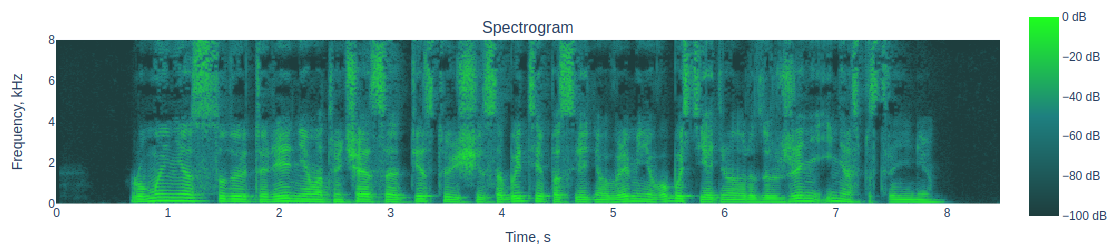
\includegraphics[width=150mm, keepaspectratio]{figures/spectogram.png}
\caption{Spectogram.}
\label{fig:TeXstudio}
\end{figure}

%  https://librosa.github.io/librosa/generated/librosa.feature.melspectrogram.html

\subsection{Neurális hálók}

A neurális hálók az emberi idegek működésének mintája alapján modellezett láncolatok. Röviden összefoglalva három különböző részt kell elképzelni. Egyik a bemenet, például egy kép esetén a pixelek, beszédfelismerés esetén az egyes időpillanatokhoz tartozó értékek vektor alakban. Spektogram esetén vektor egyes elemei a frekvenciát jelképezik és az elemek értéke pedig a hangerősséget. A neurális háló közbülső, rejtettnek, nevezett része tetszőleges méretet ölthet, mindig az előző réteg pontjaival vannak összekötve a következő réteg egyes pontjai úgy nevezett súlyok segítségével. Az újabb rétegek pontjai, amiket neuronoknak is szokás hívni, értékét az abba befutó súlyok, illetve a súlyok kiinduló pontja értékével számítódik. A háló tanítása során ezen súlyok értékét módosítjuk úgy, hogy a legoptimálisabb eredményt kapjuk. Az utolsó réteg a kimeneti réteg, ahol az eredményt kapjuk meg. A kimeneti réteg lehet regresszív, egy előre meg nem határozott, tetszőleges érték, vagy a mi esetünkben klasszifikáció, amikor előre meghatározott címkék (label-ek) valószínűségére vagyunk kíváncsiak. A legvalószínűbb címke kerül kiválasztásra válaszként.

Neurális hálót felügyelten tanítani azt jelenti, hogy először a tanítatlan hálóból kiindulva kiértékeljük egy tetszőleges bemenetre a végeredményt. Majd a végeredmény helyességétől függően változtatjuk a súlyok értékét a hálóban: azon súlyokat melyek egy rossz eredmény nagyobb valószínűségéhez járultak hozzá büntetjük, míg azokat melyek egy jó eredmény pozitív értékéhez járultnak hozzá növeljük. A büntetés mértéke is létfontosságú, hiszen fontos, hogy ne csak az adott bemenetre tudjon pontos végeredményt adni a háló, hanem általánosan is pontos legyen. 

Az E2E-hez használt leggyakoribb neurális háló réteg fajták az rekurrens (RNN) és konvolúciós (CNN) rétegek. Ez utóbbi egyik leggyakoribb felhasználási területe a különböző képfelismerő feladatok.

Az egyik legegyszerűbb réteg típus a Dense (sűrű) vagy más néven Fully Connected, ahogy a neve is mutatja a súlyokkal sűrűn vannak összekötve az egyes neuronok. Csak Dense rétegekből álló neurális háló esetén minden neuronba az előző réteg összes neuronja össze van kötve súlyokkal a következő réteg összes neuronjával.

Lényegesen összetettebb a konvolúciós réteg [5], melynél egy a teljes bemenetnél kisebb kernel-t (vagy filter-t) mozgatunk végig a bemeneten és kiértékeljük, majd összevonva egy értékké azokat a számokat, melyek a kernel-en belül vannak. A kernel-t egy megadott értékkel, a stride-al mozgatva kiértékeljük a következő, kernel által lefedett, számokat és így tovább. A konvolúció végezhető egy vagy több dimenziós bemeneten, több kernel-el is, kép esetén például három csatornás képen, ahol a piros kék és zöld értékek külön csatornákon vannak reprezentálva. Külön érdekes, hogy a bement széleit feltöltjük-e nullásokkal, ez az úgy nevezett zero padding. Ennek célja, hogy ugyan akkora legyen a kimenet, mint a padding nélküli bemenet volt. Ezen kívül is szükség lehet padding-re például egy 5x5-ös kép esetén, ha a kernel mérete 3x3 és a stride 3, akkor ki kell tölteni a kép széleit, hogy minden bemeneti értéken legalább egyszer végig menjen a kernel.

A konvolúciós hálok gyakran csökkentik a kapott bemenet méretét. A kimenet méretét a következő képlettel lehet kiszámolni, ahol ’O’ a kimenet mérete, ’W’ a bemenet mérete, ’P’ a padding mérete, ’K’ a kernel mérete és ’S’ a stride:

\begin{align}
\mathbf{O}&=\frac{\mathbf{W}-\mathbf{K}+\mathbf{2P}}{\mathbf{S}+\mathbf(1)}.
\end{align}

A rekurrens rétegek [6] egyik legérdekesebb tulajdonsága, hogy nem csupán a súlyaikat használják a neuronok kiértékeléséhez, így felhasználva a korábban tanultakat, hanem emlékeznek a korábbi bemenetekre, így azok befolyásolhatják az újabb bemenetre adott értékelést. Beszédfelismerés esetén ezt úgy is el lehet képzelni, hogy ha például elhangzik egy magánhangzó, akkor utána nagy valószínűséggel egy mássalhangzót várunk, ennek fényében, sikeres tanítás esetén, a mássalhangzókat részesíti előnyben egy azt megelőző magánhangzó után. Korábbi állapotok tehát hozzájárulnak egy újabb állapot kiértékeléséhez a rekurrens rétegben, ahogy ez a 2. ábrán is látható.
 
\begin{figure}[!ht]
\centering
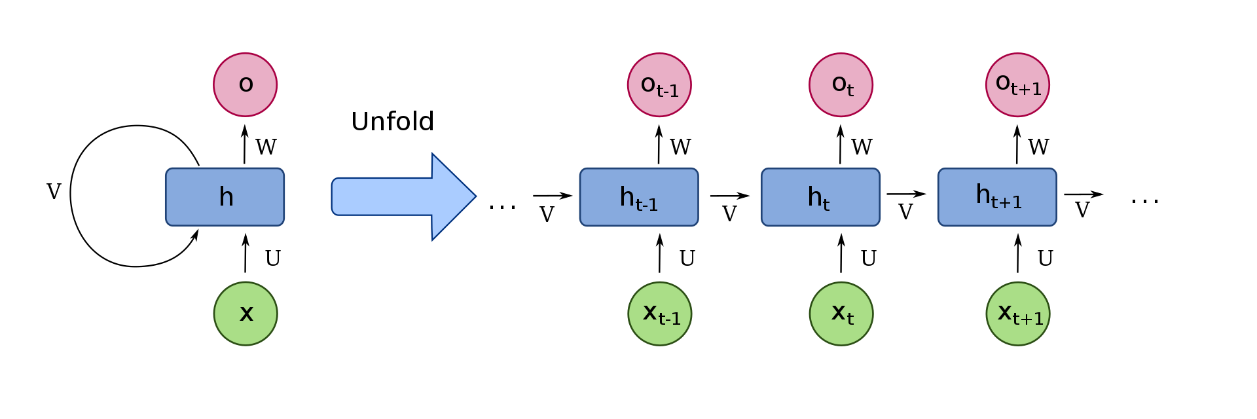
\includegraphics[width=150mm, keepaspectratio]{figures/rnn.png}
\caption{A rekurrens réteg "kigörgetve".}
\label{fig:TeXstudio}
\end{figure}

% {https://en.wikipedia.org/wiki/Recurrent_neural_network

Két altípusa a rekurrens hálóknak az LSTM és GRU (Long Short Term Memory, Gated Recurrent Unit). Ezek a típusok hasonló elveken működnek, a különbség a korábbi bemenetek újabb bementekre történő ráhatásának számítási módjában rejlik. Az LSTM [7] fő célja, hogy kijátssza a hagyományos rekurrens hálók egyik legnagyobb problémáját, azt, hogy a régebbi bemenet súlya nincs hasonló fontossággal kezelve, mint a jelenlegi bemenethez közelebbi érték. Természetesen fontos lehet egy mondat végi szót vizsgálva, hogy mi volt a szó a mondat elején, még jobban is, mint a vizsgálandó szót megelőző néhány szó. Az LSTM kapukat használ annak megelőzése céljából, hogy egy korábbi hiba elvesszen, ezáltal kezelhetetlenné téve a hiba értékelését.

A GRU egy LSTM-hez hasonló újabb fejlesztésű réteg. Egyik fő tulajdonsága, hogy kevesebb elemet tartalmaz, így kevesebb paramétert használ, csökkentve a neurális háló komplexitását.

Megemlítendő még a Bi-directional (két irányú) réteg, amely mögött az a gondolat húzódik meg, hogy ne csak a múltbéli bemenetek befolyásolják az adott bemenetünket, hanem a jövőbeliek is. Két rekurrens réteget használ, melyek ellentétes irányban haladnak egymással, így tetszőleges kiértékelésnél használhatóak a korábbi, illetve elkövetkezendő bemenetek eredményei is.

\subsection{CTC loss számítás}

A CTC funkciója a neurális háló tanításához használt loss kiszámítása, illetve a kimeneti mátrix dekódolása, a válasz kiértékelése, mely folyamán átalakítja a kimenetet a megadott címkék valószínűségi szekvenciájára. A címkék lehetnek az egyes karakterek, amik egy adott nyelvben előfordulhatnak. Ez esetben a CTC kiértékeli, hogy melyik betű vagy egyéb karakter hangzott el adott időpillanatban, adott bemenetre [8]. Ereje abban rejlik, hogy nincs szükség a kiértékelésnél a kimeneteket egyenként, karakter szinten összekötni az elvárt szöveggel, elegendő a kimeneti szöveget megadni, azt, amit kapni szeretnék a bementre. Másik fontos előnye, hogy a felismert szöveget nem szükséges külön feldolgozni, mivel átalakítja azt a végleges, feltételezett formára, például feldolgozza azt, egy hosszú hang esetén, mint az ’ú’ amikor könnyen lehet, hogy több időpillanaton keresztül is hallatszik az ’ú’ betű, de nekünk a végeredményben csak egy darab ’ú’ szükséges.

% As already discussed, we don’t want to annotate the images at each horizontal position (which we call time-step from now on). The NN-training will be guided by the CTC loss function. We only feed the output matrix of the NN and the corresponding ground-truth (GT) text to the CTC loss function. But how does it know where each character occurs? Well, it does not know. Instead, it tries all possible alignments of the GT text in the image and takes the sum of all scores. This way, the score of a GT text is high if the sum over the alignment-scores has a high value. @ https://towardsdatascience.com/intuitively-understanding-connectionist-temporal-classification-3797e43a86c + https://sid2697.github.io/Blog_Sid/algorithm/2019/10/19/CTC-Loss.html

Felmerülhet egy probléma az összevonással, amikor olyan egymást követő betűket vonunk össze, melyek a szóban külön szerepelnek, mint például a ’rabbit’ szóban. Ennek elkerülése végett bevezet a CTC egy üres karaktert, ami nem egyenlő a szóközzel, és ezt olyan időegységekhez helyezi, ahol ismerhető fel betű a megadott szótárból, karaktergyűjteményből. Az ilyen üres karakterrel elválasztott betűket nem fogja összevonni kiértékeléskor.

Kiértékelés után az ember által feldolgozható kimenet megkapásáig szükség van még dekódolásra. Az egyik legalapvetőbb dekódolási algoritmus a best path dekódolási eljárás. Két dolgot végez: kiszámolja a legvalószínűbb útvonalat a kapott kimeneti időegységeken át, majd eltávolítja az egymást követő azonos karaktereket, melyek közt nem található az üres karakter.
